\scanpage{115}%
phisme évident
\margin{\figure{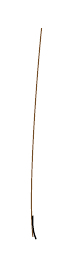
\begin{tikzpicture}[x=1cm,y=1cm]
\draw[brown!60!black,line width=.35pt] (.11,0) .. controls (.04,-.7) and (-.06,-2.1) .. (0,-2.65);
\draw[black,line width=.45pt] (0,-2.38) .. controls (-.01,-2.52) and (.01,-2.61) .. (.04,-2.68);
\end{tikzpicture}}}
\[
\handwritten{\pi}_1^t(U_t)\handwritten{\rightarrow}\handwritten{\pi}_1^t(U)
\]
(un point-base géométrique de $U_t$ étant choisi). Cet homomorphisme est \uline{surjectif}.

Démonstration. Lorsqu'on remplace $L_t$ par $L_{t'}$ générique, alors la conclusion est contenue dans le corollaire 3, en d'autres termes, si $\unsure{U|V}$ est un revêtement étale \inserted{connexe} de $U$ \deleted{tel que sa,} (satisfaisant la condition de modération en\unsure{g|v}isagée - en fait, ce n'est pas nécessaire, enx vertu de 3 ) alors sa restriction $V_{t'}$ au dessus de $U_{t'}$ est connexe. On veut prouver que sa restriction $V_t$ au dessus de $U_t$ est \inserted{\handwritten{également}} connexe. Or pour un paramètre variable sur \inserted{\handwritten{un voisinage ouvert assez petit $T$ de}} la grassmanienne \textsuperscript{$\deleted{T}$} des $L_{t'}$\handwritten{,} \deleted{et voisin de $t$, la famill} \inserted{\handwritten{la}} famille des $Y_{t'}$ est un morphisme propre et lisse $Y\handwritten{\rightarrow}T$ , et celle des $D_{t'}$ est un sous-schéma fermé \deleted{de} $\handwritten{\Delta}$ de $Y$, qui est la réunion d'un sous-schéma $\handwritten{\Delta}_1$ qui est de codi\unsure{mem|men}sion $\handwritten{\geqslant}2$ sur chaque fibre (et qui ne comp\unsure{\deleted{t}|t}e\inserted{\handwritten{\unsure{m|nt|n}}} pas, à cause du théorème de pureté relative) et d'un diviseur $\handwritten{\Delta_2}$ à croise\unsure{\`m|\`e}ents normaux relatifs. Le revêtement donné $V$ de $U$ définit un revêtement \deleted{$V$ de $Y$} $V'$ de $U'=Y-\handwritten{\Delta}$, et il\deleted{f} faut montrer que la restriction de celui-ci à la fibre géométrique de $t$ est connexe, sachant qu'il en est ainsi de sa restriction à la fibre géométrique en \unsure{\tikz[baseline=0pt,x=1pt,y=1pt]{\fill[black!80] (0,-3.7) ellipse[x radius=.55pt,y radius=.65pt];\fill[black!75] (1.6,-1.7) ellipse[x radius=.35pt,y radius=.8pt];}}$t'$, la générisation maximale de $t$. Or par la pureté, on sait que $V'$ se prolonge en un revêtement étale $V''$ de $U''=Y-\handwritten{\Delta_2}$ , et par hypothèse ce dernier est modérément ramifié sur les fibres, relativement au diviseur $\handwritten{\Delta_2}$ . La conclusion est alors une conséquence du théorème \deleted{connu} de spécialisation pour le groupe fondamental modéré, qui figure(ra) dans SGA 1 XIII (exposé de Mme Raynaud).

\uline{Remarque}7.Avec les notations de SGA 7 XVIII\handwritten{,} 6 s'applique pour tout pinceau de Lefschetz $D$ pour fournir la surjectivité de\deleted{s quotients p\unsure{a|e}r}
% The cancelled "famill" ends at the clipped right edge: no terminal e is visible.
% The two points preceding t' remain below-left of that formula; their purpose is unresolved.
% archive sheet number: 114

